\documentclass{beamer}

% Anleitung zur Klasse beamer unter: http://www.ctan.org/tex-archive/macros/latex/contrib/beamer/doc/beameruserguide.pdf

%
% Einbinden von LaTeX-Paketen
%

% Zeichenkodierung in diesem Dokument ist UTF-8
\usepackage[utf8x]{inputenc}
% Sprache des Dokuments ist Deutsch (neue Rechtschreibung)
%\usepackage{ngerman}

% es sollen Grafiken eingebunden werden
\usepackage{graphicx}

% source code
\usepackage{listings}

\usepackage{subscript}
\usepackage{xspace}

% Design Warsaw
\usetheme{Warsaw}

% abgedeckte Elemente auf einer Folie werden transparent gemacht
\setbeamercovered{transparent}

%% zu Beginn jeder Section wird folgende Folie eingefügt
\AtBeginSection[]
{
 \begin{frame}{Übersicht}
  % Übersicht: aktuelle Section (hervorgehoben) mit ubsections im Kontext anderer Sections
  \tableofcontents[currentsection,currentsubsection,hideothersubsections]
 \end{frame}
}

%% zu Beginn jeder Subsection wird folgende Folie eingefügt
%\AtBeginSubsection[]
%{
% \begin{frame}{Übersicht}
%  % Übersicht: aktuelle Section (hervorgehoben), aktuelle Subsection (hervorgehoben) im Kontext der anderen Subsections
%  \tableofcontents[currentsection,currentsubsection,subsectionstyle=show/shaded/hide]
% \end{frame}
%}

\newcommand{\ItC}{I\textsuperscript{2}C\xspace}
\newcommand{\RPi}{Raspberry~Pi\xspace}
\newcommand{\Vcc}{V\textsubscript{CC}\xspace}
\newcommand{\Vdd}{V\textsubscript{DD}\xspace}


\title{\ItC am \RPi }
\author{Guido Schmitz}
\date{Pi And More // 23. August 2012}



\begin{document}

\lstset{%
   basicstyle=\ttfamily
}


% Titelfolie
\begin{frame}[plain]
 \titlepage
\end{frame}

\begin{frame}{Overview}
 \tableofcontents
\end{frame}


\section{Was ist \ItC?}

\begin{frame}{Grundlegendes}
 \begin{itemize}
  \item \ItC = Inter-Integrated Circuit
   \begin{itemize}
    \item sprich: "I Quadrat C" oder "I Zwei C" oder "I squared C"
    \item oder auch: TWI = two wire interface (nur anderer Name)
    \item oder auch: SMBus (nur marginal technisch anders)
   \end{itemize}
  \item serieller Datenbus
   \begin{itemize}
    \item seriell = eine Datenleitung, darauf alles nacheinander
    \item Bus = mehrere Teilnehmer an gemeinsamen Leitungen
   \end{itemize}
 \end{itemize}
\end{frame}

\subsection{Physikalisch}

\begin{frame}{Leitungen}
 \begin{itemize}
  \item zwei Leitungen
   \begin{itemize}
    \item Serial Data Line (SDA)
    \item Serial Clock Line (SCL)
   \end{itemize}
  \item ein Master, mehrere Slaves (max. 112)
 \end{itemize}
 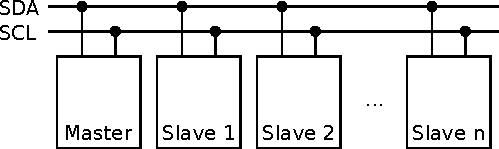
\includegraphics[width=\textwidth]{bus}
\end{frame}

\begin{frame}{Elektrisch}
 \begin{itemize}
  \item gemeinsame Referenzspannung Ground / 0V\\(auch: GND, Common, COM, V\textsubscript{SS})
  \item Versorgungsspannung \Vcc (auch: \Vdd) / hier: 3.3V
    \begin{alertblock}{Achtung}
     Viele Komponenten arbeiten mit 5V Versorgungsspannung!\\
     5V Spannung kann 3.3V Komponenten zerstören!\\
     (insbesondere das \RPi )
    \end{alertblock}
  \item aber: \ItC unkritisch (wenn richtig angeschlossen)
%  \item Ground bis \Vcc OK (max. 0.5V darüber hinaus!)
 \end{itemize}
\end{frame}

\begin{frame}{Pegel}
 \begin{itemize}
   \item Spannung = Informationszustand
    \begin{itemize}
      \item 0V = Low-Pegel = logisch 0
      \item 3.3V = High-Pegel = logisch 1
    \end{itemize}
  \item Spannung muss nicht genau passen
  \item Ganz grob gesagt: unteres Drittel Low, oberes Drittel High
 \end{itemize}
 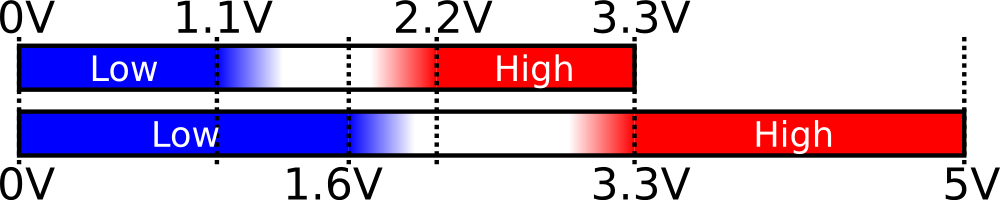
\includegraphics[width=\textwidth]{pegel.png}
\end{frame}

\begin{frame}{Pegelerzeugung}
 \begin{itemize}
   \item \ItC-Bus wird durch Pull-Up Widerstände auf 3.3V gehalten
   \item Pull-Up Widerstände hochohmig (mehrere $k\Omega$),\\im \RPi  integriert
   \item Komponenten beeinflussen Leitung erstmal nicht\\(Open-Collector, Open-Drain)
   \item Komponenten können Leitung auf Ground ziehen
 \end{itemize}
 \begin{center}
  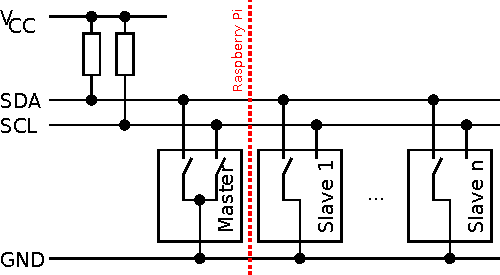
\includegraphics[width=0.6\textwidth]{bus-mit-pull}
 \end{center}
\end{frame}

\subsection{Logisch}

\begin{frame}{Kommunikation}
 \begin{itemize}
  \item Master kommuniziert abwechselnd mit einem Slave (sowohl im Sinne, dass sich Master und Slave abwechseln, als auch, dass sich Slaves untereinander abwechseln)
  \item Ein Block: 8 Bit Daten (1 Byte) und danach ein Acknowledge (ACK, von Slave)
  \item dabei: zuerst höchstwertigstes Bit
  \item SDA wird gelesen, wenn SCL kurzzeitig High
 \end{itemize}
 
\includegraphics[width=\textwidth]{bus-logisch}
% \begin{itemize}
%   \item Binär $01001011 = 2^6 + 2^3 + 2^1 + 2^0 = 75$ Dezimal
% \end{itemize}
\end{frame}

\begin{frame}{Protokoll}
 \begin{itemize}
   \item Zunächst sendet Master die Adresse des Slaves (Wer?)
    \begin{itemize}
      \item Adresse (7 Bit) kann am Slave eingestellt werden, üblicherweise erster Teil fest
      \item 8tes Bit gibt an, ob der Master eine Information lesen (1) oder schreiben (0) will
    \end{itemize}
   \item zweiter Block (vom Master) gibt an um welche Information es sich handelt (Was?)
   \item dritter Block (bei Lesen von Slave, bei Schreiben vom Master) Daten (Das!)
 \end{itemize}
\end{frame}

\section{Wie benutzen wir \ItC?}

\subsection{Der Portexpander aus dem Starterset}

\begin{frame}{MCP23016 - Allgemein}\begin{columns}
  \begin{column}{.7\textwidth}
 \begin{itemize}
  \item 16 Ein-/Ausgänge auf 2 Ports à 8 Pins
  \item jeder Pin wahlweise entweder Ein- oder Ausgang
  \item \ItC
  \item 5V
  \item schützt \RPi
  \item genaue Informationen siehe Datenblatt
  \end{itemize}
  \end{column}
  \begin{column}{.3\textwidth}
 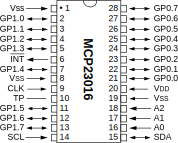
\includegraphics[width=\textwidth]{MCP23016}
  \end{column}
\end{columns}

\end{frame}

\begin{frame}{MCP23016 - \ItC}\begin{columns}
\begin{column}{.7\textwidth}
 \begin{itemize}
  \item Adresse: 0100XXX (erste vier Bits fest)\\Anschlüsse A2,A1,A0 bestimmen letzte drei Bits
  \item Welche Register (s.o. Was?):
   \begin{tabular}{|l|l|}\hline
    0x00 & Port 0, Werte\\\hline
    0x01 & Port 1, Werte\\\hline
    0x06 & Port 0, Richtung\\\hline
    0x07 & Port 1, Richtung\\\hline
   \end{tabular}
   
   (Richtung: 0=Ausgang, 1=Eingang)
 \end{itemize}
 \end{column}
  \begin{column}{.3\textwidth}
 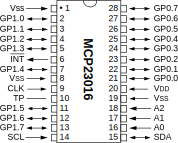
\includegraphics[width=\textwidth]{MCP23016}
  \end{column}
 \end{columns}
\end{frame}

\subsection{Beispielaufbau}

\begin{frame}{Hinweis}
 \begin{alertblock}{Achtung!}
  Hinweise auf dem Beipackzettel beachten!\\
  Erst denken und nochmal überprüfen, dann erst anschalten!
 \end{alertblock}
\end{frame}

\begin{frame}{Beispielschaltung (1)}
 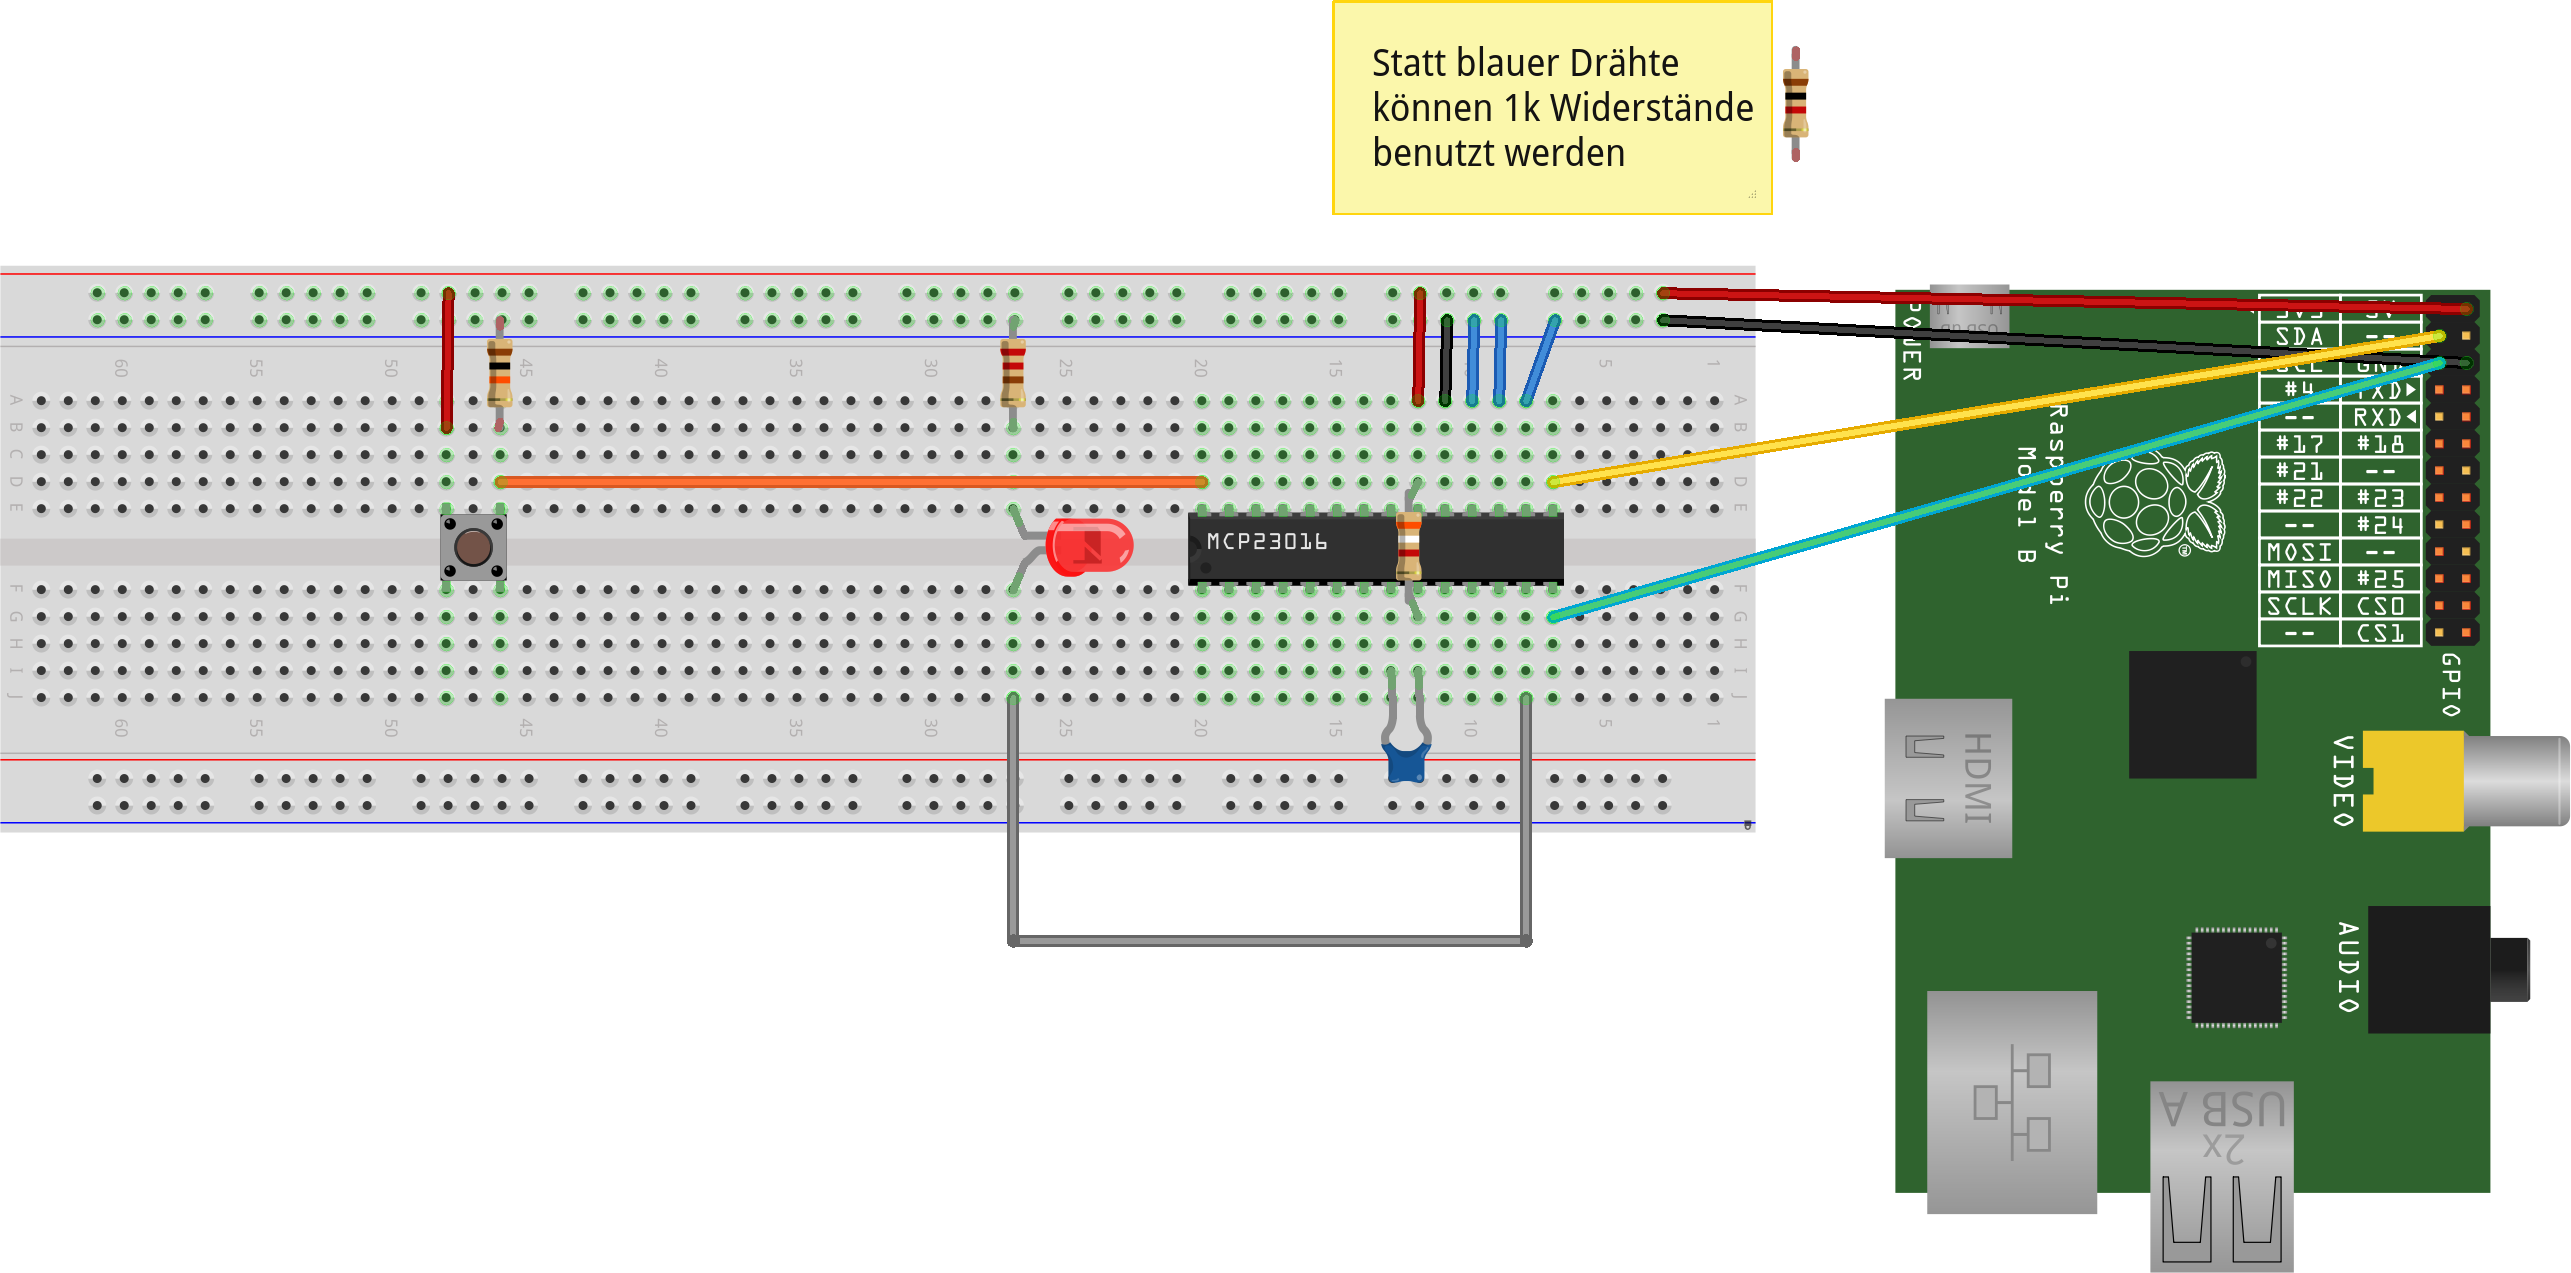
\includegraphics[width=\textwidth]{testaufbau.png}
\end{frame}

\begin{frame}{Beispielschaltung (2)}
 \begin{itemize}
   \item \RPi
   \item Portexpander MCP23016
    
  \item LED (abgeflachte Seite ist -)
  \item Sonstiges: Vorwiderstand für LED, Widerstand + Kondensator für MCP23016
 \end{itemize}
\end{frame}



\subsection{Einrichtung (Software)}

\begin{frame}[fragile]{Vorbereitung des \RPi  (1)}
 \begin{itemize}
   \item Vorraussetzung: installiertes Raspbian
   \item Installation der Software:
    \lstset{language=bash}
    \begin{lstlisting}
sudo apt-get update
sudo apt-get install python-smbus i2c-tools
    \end{lstlisting}
  \item in \lstinline|/etc/modprobe.d/raspi-blacklist.conf| die Zeile
    \begin{lstlisting}
blacklist i2c-bcm2708
    \end{lstlisting} ändern in \begin{lstlisting}
#blacklist i2c-bcm2708
    \end{lstlisting}
 \end{itemize}
\end{frame}
 
\begin{frame}[fragile]{Vorbereitung des \RPi  (2)}
 \begin{itemize}
  \item in \lstinline|/etc/modules| folgende Zeilen ergänzen:
    \begin{lstlisting}
i2c-dev
i2c-bcm2708
    \end{lstlisting}
  \item \ItC für Benutzer freischalten:
    \begin{lstlisting}
sudo adduser pi i2c
    \end{lstlisting}
  \item Neustarten
 \end{itemize}
\end{frame}

\subsection{Inbetriebnahme}

\begin{frame}[fragile]{Python}
 Ein kleines Python-Programm:
 \lstset{language=Python}
 \begin{lstlisting}
# I2C laden
import smbus
bus = smbus.SMBus(0)
# Port 1: erster Pin als Ausgang
bus.write_byte_data(0x20, 0x07, 0b11111110)
# Port 1: erster Pin auf High
bus.write_byte_data(0x20, 0x01, 0b00000001)
# Port 1: erster Pin auf Low
bus.write_byte_data(0x20, 0x01, 0b00000000)
# Port 0: Pins abfragen
x = bus.read_byte_data(0x20, 0x00)
 \end{lstlisting}
 Tipp: kann man direkt in Python eintippen (Befehl: \lstinline[language=bash]|python|)
\end{frame}

\begin{frame}[plain]
        \begin{center}
        \huge Fragen?
    \end{center}
        \tableofcontents
\end{frame}


\end{document}
